\documentclass[UTF8]{article}
\usepackage{ctex}
\usepackage{graphicx}
\usepackage{amsmath}
\usepackage{amssymb}    % \therefore \because
\usepackage{bm}     % \bm 用于数学字符加粗



\begin{document}
    \title{Note of Linear Algebra}
    \author{Yzy}
    \maketitle
    \tableofcontents

    \section{Chapter1---vector and linear combination}
    
    scalar multiplication(标量乘法): 2\textbf{\textit{v}}
    \quad
    vector addition(矢量加法): \textbf{\textit{vw}}
    \\
    \textit{xy} plane(二维平面) \quad \textit{xyz} space(三维空间)
     
    $$
    \textit{列向量v} =
    \begin{bmatrix}
        1 \\ 1 \\ -1  
    \end{bmatrix}
    \textit{转置(transpose)}\rightarrow
    \textit{行向量v} = 
    \begin{bmatrix}
        1 & 1 & -1
    \end{bmatrix}
    $$

    假设有三维向量\textbf{\textit{u,v,w}},系数$c,d,e$,在不考虑它们是零向量的情况下:
    \begin{enumerate}
            \item $c\bm{u}+d\bm{v}+e\bm{w}$ 覆盖整个三维空间
            \item $c\bm{u}+d\bm{v}$ 覆盖三维空间中的某一个平面
            \item $c\bm{u}$ 覆盖三维空间中的某一条直线
    \end{enumerate}
    故欲使$c\bm{u}+d\bm{v} = \bm{w}$ 有解,$\bm{w}$必须在$c\bm{u}+d\bm{v}$构成的平面上!
    \\
    整数 whole numbers \quad 等间距点 equally spaced points
    \\
    几何 geometric \quad lattice 点阵
    \\
    点积 dot product(内积 inner product): $\bm{v} \cdot \bm{w}$ 即为对应元素相乘再求和!
    \\
    长度$\Vert \bm{v} \Vert = \sqrt{\bm{v \cdot v}} = (v_{1}^{2}+v_{2}^{2}+\cdots+v_{n}^{2})^{1/2}$ 
    \\
    单位向量(unit vector) $\bm{u} = \frac{\bm{v}}{ \Vert \bm{v} \Vert}$ 且与$\bm{v}$同方向! \\
    \textbf{方阵:}
    \begin{itemize}
        \item 非奇异矩阵(可逆矩阵) nonsingular(invertible) matrix
        \item 奇异矩阵(非可逆矩阵) singular matrix
    \end{itemize}

    \section{Chapter2---Solving Linear Equations}
    \subsection{vectors and linear equations}
    $\bm{A}_{m\times n}\bm{x}_{n \times 1}=\bm{b}$ 分别从行和列的角度来看
    \begin{itemize}
        \item 行:从m个方程n个未知数得到的“平面”是处于\textbf{n维空间}
        \item 列:从n列且行数为m的列向量得到的线性组合是处于\textbf{m维空间}
    \end{itemize}

    \textbf{矩阵乘法}(行图像形式):
    $$
    \begin{bmatrix}
        2 & 0 \\
        0 & 5
    \end{bmatrix}
    \begin{bmatrix}
        row1 \\
        row2
    \end{bmatrix}
    = 
    \begin{bmatrix}
        2*row1 + 0*row2 \\
        0*row1 + 5*row2
    \end{bmatrix}
    =
    \begin{bmatrix}
        2*row1 \\
        5*row2
    \end{bmatrix}
    $$
    $$
    AB =
    \begin{bmatrix}
       \bm{a_1} \\ \bm{a_2} 
    \end{bmatrix}
    B = 
    \begin{bmatrix}
        \bm{a_1} \cdot B \\ \bm{a_2} \cdot B
    \end{bmatrix}
    =
    \begin{bmatrix}
        a_{11} * \bm{b_1} + a_{12} * \bm{b_2} \\ a_{21} * \bm{b_1} + a_{22} * \bm{b_2}
    \end{bmatrix}
    $$
    这里$\bm{a_i}$与$\bm{b_i}$均为行向量。\\
    用这种乘法可以快速理解左乘置换矩阵$P_{ij}$为什么能改变行的顺序\\
    $$
    AB=A
    \begin{bmatrix}
        \bm{b_1} & \bm{b_2} & \bm{b_3}
    \end{bmatrix}
    =
    \begin{bmatrix}
        A\bm{b_1} & A\bm{b_2} & A\bm{b_3}
    \end{bmatrix}
    =
    \begin{bmatrix}
        \bm{a_1} \\ \bm{a_2} \\ \bm{a_3}
    \end{bmatrix}
    B=
    \begin{bmatrix}
        \bm{a_1}B \\ \bm{a_2}B \\ \bm{a_3}B
    \end{bmatrix}
    $$ 这里$\bm{b_i}$为列向量,$\bm{a_i}$为行向量。\\
    \textbf{列图像形式}: 矩阵A乘矩阵B的\textbf{每列},得到的结果AB的每一列都是\textbf{A的列的线性组合}。\\
    \textbf{行图像形式}: 矩阵A的\textbf{每行}乘矩阵B,则AB的每一行均为\textbf{B的行的线性组合}
    \textbf{列乘行形式}:
    $$
    \begin{bmatrix}
        col1 & col2 & col3 \\ . & . & . \\ . & . & .
    \end{bmatrix}
    \begin{bmatrix}
        row1 \cdots \\
        row2 \cdots \\
        row3 \cdots 
    \end{bmatrix}
    = (col1)(row1) + (col2)(row2) + (col3)(row3)
    $$

    \textbf{矩阵乘法在邻接矩阵中应用 2.4 worked example A} \\
    adjacency matrix
    $$
    \bm{S} =
    \begin{bmatrix}
        0 & 1 & 1 & 0\\
        1 & 0 & 1 & 1\\
        1 & 1 & 0 & 1\\
        0 & 1 & 1 & 0
    \end{bmatrix}
    $$
    其中,$(S^2)_{ij}$表示结点i与结点j之间,步长为2的路径数目。\\
    $(S^2)_{ij}=$(row $i$ of $S$)$\cdot$(column $j$ of $S$)$=s_{i1}s_{1j}+s_{i2}s_{2j}+s_{i3}s_{3j}+s_{i4}s_{4j}$

    \subsection{矩阵的LU分解}
    $(E_{32}E_{31}E_{21})A=U \rightarrow A = (E_{21}^{-1}E_{31}^{-1}E_{32}^{-1})U \rightarrow A=LU$
    \\
    $\bm{L, U}$分别是\textbf{下三角矩阵,上三角矩阵}。
    \\
    又因为
    $$
    U=
    \begin{bmatrix}
        d_1 & & &\\
         & d_2 & &\\
         &  & \ddots & \\
         &  & & d_n
    \end{bmatrix}
    \begin{bmatrix}
        1 & u_{12}/d_{1} & u_{13}/d_{1} & \cdot \\
          & 1 & u_{23}/d_2 & \cdot \\
          &   & \ddots & \vdots \\
          &   &   & 1
    \end{bmatrix}
    $$
    所以也可以写成$A=LDU$,$D$为主元对角矩阵,$U$主对角线为1。

    \subsection{转置(transposes)与置换(permutations)}
    \textbf{转置transpose}: $(A^T)_{ij} = A_{ij}$\\
    若LU分解中的A是\textbf{对称的(symmetric)},则记为$S$,且分解过程可写成$A=LDU \rightarrow S=LDL^T$,其中$U=L^T$
    \\
    \textbf{置换permute以及置换矩阵permutation matrices P}\\
    P即是对\textbf{单位矩阵I}进行\textbf{行变换或列变换}得到的矩阵。而不是只进行交换两行或两列的初等矩阵!\\
    $P^{-1} = P^T$ 且 $PP^T = I$

    \textbf{提前做行交换再进行分解PA=LU}\\
    若A是可逆的,且A在消元过程中需要做行交换,则可以在分解之前利用P提前做行变换$\rightarrow PA$,
    因此可以得到$PA=LU$

    \section{向量空间 Space of Vectors}
    标准n维空间$R^n$可以理解为:$R \times R \times \dots \times R$,即n个R的笛卡尔积,即n维向量的所有可能情况!
    \\
    \textbf{向量空间}必须满足的规则:该空间对\textbf{数乘,加法}封闭,即通过这两种操作所产生的向量依然在此空间。
    \\
    注意:一个在三维空间中通过(0,0,0)的平面,是该三维空间的子空间,但不是$\bm{R^2}$。\\
    \subsection{子空间subspaces}
    同样对\textbf{数乘,加法}封闭,且\textbf{必须包含零向量}(当c=0时,数乘$c \bm{v}=\bm{0}$)
    \\
    关于$\bm{R^3}$的所有子空间:
    \begin{itemize}
        \item 所有过(0,0,0)的平面
        \item 所有过(0,0,0)的直线
        \item $\bm{Z}$原点,或零向量(0,0,0)
        \item 整个空间$\bm{R^3}$
    \end{itemize}
    \subsection{列空间column space}
    基于矩阵A的\textbf{列向量的所有线性组合}构成了列空间,这些组合是所有可能的$A\bm{x}$,它们填满了\textbf{列空间}$\bm{\mathcal{C}}(A)$。
    \\
    $A_{m\times n}$有n个列向量,每个列向量有m维。故,这些列向量属于$\bm{R^m}$空间。A的列空间是$\bm{R^m}(not \bm{R^n})$的\textbf{一个子空间}(满足子空间要求)!
    \\
    这一个概念至关重要,因为它\underline{将$A\bm{x}=\bm{b}$问题转化为$\bm{b}$是否能由$A$的列向量线性表出的问题}!
    \\
    方程组$A\bm{x}=\bm{b}$有解当且仅当向量$\bm{b}$处于$A$的列空间中!\\
    $A, \quad [A \quad AB]$\textbf{有相同的列空间},因为$AB$\textbf{实质也是A的列向量的线性组合}!
    \\
    \subsection{子空间的交、并、和}
    \textbf{子空间的并}:$P\cup L$,如平面P和一条直线L之间,它们之间的并集对线性运算(加法)不封闭.所以子空间的并不是一个向量空间!
    \\
    \textbf{子空间的交}:$P\cap L$,平面P和直线L相交于原点,显然是$\bm{R^3}$的子空间。\\
    \textbf{推广:}任意两个子空间的交集,仍是子空间!\\
    \textbf{子空间的和:P+L}各取一条向量,相加之后的向量处于平面和直线之间!脱离了并集构成的空间.若两个子空间均为直线,则它们的和为一个过原点的平面。\textbf{子空间的加法不仅包含它们的并,也包含了它们的线性组合}。
    例如:并就是集合的并集,而和是在并的基础之上把所有线性运算的结果都包含进去。比如x轴并y轴就是那两个轴,而它们的和得把空的地方都补上,是整个平面。
    \\
    $dim(S)+dim(U) = dim(S\cap U) + dim(S+U)$
    \subsection{零空间Nullspaces}
    零空间Nullspaces $\bm{N}(A)$, 行最简矩阵(reduced row echelon form) $R = \bm{rref}(A)$
    ,$\bm{N}(A)=\bm{N}(R)$
    \\
    $A_{m\times n}\bm{x}=\bm{0}$的\textbf{所有解向量的线性组合}构成了零空间$\bm{N}(A)$, 因为解向量$\bm{x}$是n维的,所以该零空间是n维空间$\bm{R}^n$的一个\textbf{子空间}。
    \\
    $m>n$对方程组添加新的方程(行),会对解向量变得更加严格,原零空间不会变大!\\
    $n>m$方程组至少有一个自由变量,即至少有一个非零解。\\
    零空间是子空间,且它的\textbf{维度是自由变量的个数}(非主元pivot个数,即列数n减去主元个数)

    \subsection{秩rank}
    rank of A : 主元pivot数目,记为$r$。\quad 每个自由列都是主列的线性组合!
    \begin{itemize}
        \item A有r个线性无关列(行)
        \item A的列空间(行空间)的维度是r
        \item n-r是$A_{m\times n}\bm{x}=\bm{0}$的解空间的维度
    \end{itemize}
    这里说的\textbf{维度}$\rightarrow$构成向量空间的\textbf{基的线性无关向量的个数}!\\
    \textbf{特殊的---秩为1的矩阵}\\
    秩为1的矩阵可以写成(列向量乘行向量): $A=\bm{uv}^T$. \quad 如:
    $$
    \begin{bmatrix}
        1 & 3 & 10\\
        2 & 6 & 20\\
        3 & 9 & 30
    \end{bmatrix}
    =
    \begin{bmatrix}
        1\\
        2\\
        3
    \end{bmatrix}
    \begin{bmatrix}
        1 & 3 & 10
    \end{bmatrix}
    $$
    $A\bm{x}=\bm{0}, \rightarrow \bm{u(v}^T\bm{x})=\bm{0} \rightarrow \bm{v}^T\bm{x}=\bm{0}$
    可以看出,行(列)空间是一条直线,且解空间中所有的向量都要垂直于向量$\bm{v}^T$,故解空间是一个垂直于向量的平面$\bm{v}^T$。
    \\
    \textbf{A的按秩分解规律}\\
    $A_{m\times n}, r(A)=r$,欲将A分解为$(m\times r)(r \times n)$的矩阵:\\
    $A = (A \textbf{的主元列})(R的\textbf{前}r\textbf{行})=(COL)(ROW)$, R为A的行最简矩阵。把这个过程看成是\textbf{A的主元列的线性组合},R前r行包含了单位阵I和自由变量列。

    \subsection{线性相关性Independence,基Basis,维数Dimension}
    一个空间的维度dimension是组成这个空间的基的线性无关的向量个数!$\mathbf{R}^{n}$的\textbf{维数是n, 且向量的维数也是n}\\
    $\mathbf{C}(A)$--->$r$维;$\mathbf{N}(A)$--->$n-r$维。\\
    \subsection{矩阵空间Matrix Spaces 5th P182}
    一个向量空间M包含了所有2*2矩阵,它的维度是4!\quad 它的一个\textbf{基}为:
    $A_{1}, A_{2}, A_{3}, A_{4}=\left[\begin{array}{ll}{1} & {0} \\ {0} & {0}\end{array}\right],\left[\begin{array}{ll}{0} & {1} \\ {0} & {0}\end{array}\right],\left[\begin{array}{ll}{0} & {0} \\ {1} & {0}\end{array}\right],\left[\begin{array}{ll}{0} & {0} \\ {0} & {1}\end{array}\right]$

    \subsection{函数空间Function Spaces}
    二阶微分方程$\frac{d^{2} y}{d x^{2}}+y=0$只考虑实数范围,有两个特解:$y=\sin x and y=\cos x$
    \\
    它的通解即为这两个特解的线性组合:$\mathrm{y}=c_{1} \cos \mathrm{x}+c_{2} \sin \mathrm{x}_{\circ}$
    \\
    这类似于零空间,将解看成空间中的元素,全部解构成解空间,满足线性运算封闭条件。\textbf{维数为2}\\
    $y^{\prime \prime}=0$的解空间即类似零空间,为$y=c x+d$。\\
    而$y^{\prime \prime}=2$不形成子空间,因为右边的2不是0,无法形成零空间。它的全部解为特解$y(x)=x^{2}$加上零空间$y=c x+d$
    即为$y(x)=x^{2}+c x+d$。\\
    \textbf{空间}$\bm{Z}$只包含零向量,它的维度为$\bm{0}$。空集empty set是$\bm{Z}$的一个基。
    若将一个零向量加入到一个基中,则会\textbf{破坏基中的线性无关性}。\\

    \subsection{四个基本子空间}
    \begin{itemize}
        \item \textbf{关联矩阵}incidence matrix 可以用来表示有向图,有环则说明结点代表的向量是\textbf{线性相关的},有树则\textbf{线性无关}
        \item 列空间$\mathcal{C}(A)$,行空间$\mathcal{C}(A^T)$,零空间$\mathcal{N}(A)$,左零空间$\mathcal{C}(A^T)$
    \end{itemize}
    若求出了A的行阶梯或行最简矩阵R,再求出所用的行变换矩阵E,则可以通过E来求出左零空间的基,即$A^Tx=0$的解。
    \\
    $$\boldsymbol{E} \boldsymbol{A}=\boldsymbol{R}
    =
    \left[\begin{array}{rrr}{1} & {0} & {0} \\ {-1} & {1} & {0} \\ {-2} & {-2} & {1}\end{array}\right]
    \left[\begin{array}{lll}{1} & {0} & {3} \\ {1} & {1} & {7} \\ {4} & {2} & {20}\end{array}\right]
    =
    \left[\begin{array}{lll}{1} & {0} & {3} \\ {0} & {1} & {4} \\ {0} & {0} & {0}\end{array}\right]
    $$
    因为$A^T$的列是$A$的行,所以可以从上面直接看出3-2=1,即解空间维数唯一。且R的第三行为零向量,由E的第三行乘上A的每行向量得到!
    \\
    所以有$A^T({row_3(E)}^T)=\textbf{0}$,\textbf{所以可以不用再求解一遍}$A^Tx=0$,\textbf{可以直接从E和R看出左零空间的基!}
    \\
    故有:若$\boldsymbol{E} \boldsymbol{A}=\boldsymbol{R}$, 则E的\textbf{后$\bm{m-r}$行}是$A$的左零空间的基!
    \\
    \textbf{注意}:AB的所有行都是B行的组合,因此AB的行空间包含在(可能等于)B的行空间中,所以rank(AB)<rank(B)。
    AB的所有列是A的列的组合,因此AB的列空间包含在(可能等于)A的列空间中,所以rank(AB)<rank(A)。
    \\
    \textbf{若A,B的四个基本子空间都相同,则}$\bm{B=cA,c\neq 0}$
    \subsection{每个秩r的矩阵=r个秩1矩阵之和}
    对应上面矩阵$\boldsymbol{E} \boldsymbol{A}=\boldsymbol{R}$\\
    $A=\left[\begin{array}{lll}{u_{1}} & {u_{2}} & {u_{3}}\end{array}\right]\left[\begin{array}{c}{v_{1}^{\mathrm{T}}} \\ {v_{2}^{\mathrm{T}}} \\ {\text { zero row }}\end{array}\right]=u_{1} v_{1}^{\mathrm{T}}+u_{2} v_{2}^{\mathrm{T}}=(\text { rank } 1)+(\text { rank } 1)$
    A的主元列$\bm{u_1,u_2}$, R的前r行(主元行)$\bm{v_{1}^{T}, v_{2}^{T}}$.\\

    \section{正交性orthogonality}
    \subsection{4个子空间的正交性}
    当b在列空间之外时(当我们想要求解Ax = b而不能这样做时)那么$A^T$的这个零空间就会自成一体。 它包含“最小二乘”解决方案中的误差$e = b-Ax$。最小二乘法是本章线性代数的关键应用。
    \\
    同一个向量空间的两个子空间V,W有 \textbf{V与W是正交的}:$\boldsymbol{v}^{\mathrm{T}} \boldsymbol{w}=0$ for all $\boldsymbol{v}$ in $\boldsymbol{V}$ and all $\boldsymbol{w}$ in $\boldsymbol{W}$
    \\
    注意:一定是子空间中的每个向量!比如三维空间中的两个垂直的平面,因为它们的交线不能垂直于自己,所以这两个平面不是正交的!
    \\
    若有一个向量能同时处于两个正交子空间中,则这个向量必定是\textbf{零向量},零向量垂直于自己。\\
    当$\operatorname{dim} V+\operatorname{dim} W>\operatorname{dim}(\text { whole space })$,$V$和$W$\textbf{不可能正交}!
    \\
    Every vector $x$ in the nullspace is perpendicular to every row of $A,$ because $A x=0$ .\\
    The nullspace $N(A)$ and the row space $C\left(A^{T}\right)$ are orthogonal subspaces of $\mathbf{R}^{n}$ .$C(A^T) \perp N\left(A \right)$
    \\
    2 proof:
    \begin{itemize}
        \item $A \boldsymbol{x}=\left[\begin{array}{c}{\operatorname{row} 1} \\ {\vdots} \\ {\operatorname{row} m}\end{array}\right][\boldsymbol{x}]=\left[\begin{array}{c}{0} \\ {\vdots} \\ {0}\end{array}\right]$,Every row has a zero dot product with $\bm{x}$. Then $\bm{x}$ is also perpendicular
to every combination of the rows.
        \item 行空间中的向量是行的线性组合$A^T\bm{y}$,\quad $\bm{x}$则是零空间的向量,则有$\boldsymbol{x}^{\mathrm{T}}\left(A^{\mathrm{T}} \boldsymbol{y}\right)=(A \boldsymbol{x})^{\mathrm{T}} \boldsymbol{y}=\mathbf{0}^{\mathrm{T}} \boldsymbol{y}=0$.
    \end{itemize}
    Every vector $y$ in the nullspace of $A^{\mathrm{T}}$ is perpendicular to every column of $A$\\
    The left nullspace $N\left(A^{\mathrm{T}}\right)$ and the column space $C(A)$ are orthogonal in $\mathbf{R}^{m}$, $C(A) \perp N\left(A^{\mathrm{T}}\right)$.
    \\
    \subsection{正交补orthogonal complements}
    定义:一个子空间V的\textbf{正交补包含了每一条垂直于V的向量},这个正交空间记为:$V^\perp$.\\
    例子:零空间是行空间的正交补,每一条垂直于行空间的向量都满足$A\bm{x}=\bm{0}$,且均处于零空间中。它们满足$r+(n-r)=n$。列空间和左零空间同理!
    \\
    \begin{itemize}
        \item 零空间$\mathbf{N}(A)$是行空间$\boldsymbol{C}\left(A^{\mathrm{T}}\right)\left(\text { in } \mathbf{R}^{n}\right)$的正交补---$\mathbf{N}(A) = (\boldsymbol{C}\left(A^{\mathrm{T}}\right))^\perp$
        \item 左零空间$N\left(A^{\mathrm{T}}\right)$是列空间$C(A)\left(\text { in } \mathbf{R}^{m}\right)$的正交补---$\mathbf{N}(A^T) = (\boldsymbol{C}\left(A\right))^\perp$
    \end{itemize}
    正交补的两个子空间的\textbf{交集只能为}$\bm{0}$。 \\
    \textbf{互补的含义}\\
    \textbf{每个向量$\bm{x}$都可以分成行空间分量$\bm{x}_r$和零空间分量$\bm{x}_n$}.\\
    $\boldsymbol{x}=\boldsymbol{x}_{r}+\boldsymbol{x}_{n}$,\quad $A \boldsymbol{x}=A \boldsymbol{x}_{r}+A \boldsymbol{x}_{n}$.
    \begin{itemize}
        \item 零空间分量变成零向量$A \boldsymbol{x}_{n}=\mathbf{0}$
        \item 行空间分量变成了列空间向量$A \boldsymbol{x}_{r}=A \boldsymbol{x}$
    \end{itemize}
    这说明了,一个向量左乘一个矩阵A,会变成列空间中的一个向量!而且:列空间中的向量$\bm{b}$来自有且仅有一个行空间中的向量$\bm{x}_r$。
    \\
    \begin{itemize}
        \item 一个原空间S可以划分为行空间和零空间,或者列空间和左零空间,\textbf{一般地说可以划分为两个正交补子空间!}
        \item 正交补子空间空间的特点是\textbf{两个正交子空间维度之和为dim(S)}
    \end{itemize}
    \textbf{正交补子空间的基底构成了原空间的基底!}
    由行空间和零空间的基底可得,$r+(n-r)=n$个向量,这r个向量是线性无关的,因此它们构成了$\mathbf{R}^{n}$。
    \\
    如果所有n个向量的组合给出$\boldsymbol{x}_{r}+\boldsymbol{x}_{n}=\mathbf{0}$,则$\boldsymbol{x}_{r}=-\boldsymbol{x}_{n}$在两个子空间中。所以$\boldsymbol{x}_{r}=\boldsymbol{x}_{n}=\bm{0}$。行空间基底和零空间基底的所有系数必须为零。 这证明了n个向量的线性无关性。
    \\
    练习:若$A^{\mathrm{T}} A \boldsymbol{x}=0$ then $A \boldsymbol{x}=\mathbf{0}$.\quad 因为$A \boldsymbol{x}$处于A的列空间中,同时也处于$A^T$的零空间中,即A的左零空间中,故$A \boldsymbol{x}$只能是\textbf{零向量}。

    \subsection{投影projections}
    \textbf{投影矩阵Projection matrix}\\
    $P_{1}=\left[\begin{array}{lll}{0} & {0} & {0} \\ {0} & {0} & {0} \\ {0} & {0} & {1}\end{array}\right]$\quad 将向量$\bm{b}$投影到z轴
    \\
    $\boldsymbol{p}_{1}=P_{1} \boldsymbol{b}=\left[\begin{array}{ccc}{0} & {0} & {0} \\ {0} & {0} & {0} \\ {0} & {0} & {1}\end{array}\right]\left[\begin{array}{l}{x} \\ {y} \\ {z}\end{array}\right]=\left[\begin{array}{l}{\mathbf{0}} \\ {\mathbf{0}} \\ {z}\end{array}\right]$
    \\
    $P_{2}=\left[\begin{array}{lll}{1} & {0} & {0} \\ {0} & {1} & {0} \\ {0} & {0} & {0}\end{array}\right]$\quad 将向量$\bm{b}$投影到$xy-plane$
    \\
    $p_{2}=P_{2} b=\left[\begin{array}{lll}{1} & {0} & {0} \\ {0} & {1} & {0} \\ {0} & {0} & {0}\end{array}\right]\left[\begin{array}{l}{x} \\ {y} \\ {z}\end{array}\right]=\left[\begin{array}{l}{x} \\ {y} \\ {0}\end{array}\right]$
    \\
    投影后的z轴与xy平面是正交补,$dim(z axis) + dim(xy-plane) = dim(\bm{R}^3)$.所以此三维空间中的每个向量$\bm{b}$都可以由这两个子空间的向量构成。
    \\
    即$\boldsymbol{p}_{1}+\boldsymbol{p}_{2}=\boldsymbol{b}$,投影矩阵也有$P_{1}+P_{2}=I$。
    \\
    \textbf{利用$A\bm{x}=\bm{b}$是将x投影至A的列空间这一概念},可以解释上述投影原理:将z轴和xy-plane的基分别放至一个对应$\bm{R}^m$空间的$m\times m$矩阵$P_1,P_2$中,这两个矩阵分别乘上向量$\bm{b}$即表示将向量$\bm{b}$投影至它们的列空间,正好分别对应z轴和xy-plane。
    \subsubsection{b投影到直线a上}
    $\bm{b}$投影到$\bm{a}$上的投影向量为$\bm{p}$,必有$\bm{p}=\widehat{x} \bm{a}$,其中$\hat{x}$是倍数。
    \\
    误差向量$\bm{e}=\bm{b}-\bm{p}=\bm{b}-\widehat{x} \bm{a}$,且$\bm{e} \perp \bm{a}$。\quad 利用它们点乘为0求出倍数:
    \\
    $a \cdot(b-\widehat{x} a)=0$--->$a \cdot b-\widehat{x} a \cdot a=0$--->$\widehat{\boldsymbol{x}}=\frac{\boldsymbol{a} \cdot \boldsymbol{b}}{\boldsymbol{a} \cdot \boldsymbol{a}}=\frac{\boldsymbol{a}^{\mathrm{T}} \boldsymbol{b}}{\boldsymbol{a}^{\mathrm{T}} \boldsymbol{a}}$
    \\
    所以,向量$\bm{b}$在$\bm{a}$上的投影为$\boldsymbol{p}=\widehat{\boldsymbol{x}} \boldsymbol{a}=\frac{\boldsymbol{a}^{\mathrm{T}} \boldsymbol{b}}{\boldsymbol{a}^{\mathrm{T}} \boldsymbol{a}} \boldsymbol{a}$。
    \\
    \textbf{再求所用的投影矩阵P}\\
    $\boldsymbol{p}=\boldsymbol{a} \widehat{\boldsymbol{x}}=\boldsymbol{a} \frac{\boldsymbol{a}^{\mathrm{T}} \boldsymbol{b}}{\boldsymbol{a}^{\mathrm{T}} \boldsymbol{a}}=P \boldsymbol{b}$
    \quad $\therefore P=\frac{a a^{\mathrm{T}}}{a^{\mathrm{T}} a}$, $rank(P)=1$\\
    $P^{2}=P$,投影两次到P的列空间中还是一样的。\\
    \textbf{矩阵${I-P}$}同样对向量$\bm{b}$作投影,$(I-P) \boldsymbol{b}=\bm{b}-\bm{p}=\bm{e}$,这说明该矩阵将b投影到b的垂直部分e。
    \\
    \textbf{当矩阵P将b投影至一个子空间V中,I-P会将b投影到一个垂直于V的子空间W中},上述的I-P将b投影至垂直于向量$\bm{a}$的平面中!
    \subsubsection{b投影到子空间上}
    假设有n个向量$\boldsymbol{a}_{1}, \ldots, \boldsymbol{a}_{n}$ in $\mathbf{R}^{m}$,且它们线性无关,$A=[\boldsymbol{a}_{1}, \ldots, \boldsymbol{a}_{n}]$。
    \\
    找到最接近$\bm{b}$的线性组合$\boldsymbol{p}=\widehat{x}_{1} \boldsymbol{a}_{1}+\cdots+\widehat{x}_{n} \boldsymbol{a}_{n}=A \widehat{\boldsymbol{x}}$即为将$\bm{b}$投影至$\bm{a's}$扩展的子空间。
    \\
    若n=1,则说明这是投影至一条直线上,$\widehat{x}=\boldsymbol{a}^{\mathrm{T}} \boldsymbol{b} / \boldsymbol{a}^{\mathrm{T}} \boldsymbol{a}$
    \\
    若n>1,则说明这是投影至一个子空间上,则最佳的组合系数是$\widehat{\boldsymbol{x}}=\left(\widehat{x}_{1}, \dots, \widehat{x}_{n}\right)$
    \\
    同样有误差向量$\bm{e}=\bm{b}-\bm{p}=\bm{b}-A \widehat{x}$垂直于$\bm{a's}$构成的子空间,即$\perp \boldsymbol{a}_{1}, \ldots, \perp \boldsymbol{a}_{n}$,利用点积为0构造等式:
    \\
    $$
    \begin{array}{c}
        \boldsymbol{a}_{1}^{\mathrm{T}}(\boldsymbol{b}-A \widehat{\boldsymbol{x}})=0\\
        \vdots  \\
        \boldsymbol{a}_{n}^{\mathrm{T}}(\boldsymbol{b}-A \widehat{\boldsymbol{x}})=0
    \end{array}
    \rightarrow
    \left[\begin{array}{c}{-\boldsymbol{a}_{1}^{\mathrm{T}}-} \\ {\vdots} \\ {-\boldsymbol{a}_{n}^{\mathrm{T}}-}\end{array}\right]\Bigg[\boldsymbol{b}-A \widehat{\boldsymbol{x}}\Bigg]=\Bigg[\mathbf{0}\Bigg]
    \rightarrow
    A^{\mathrm{T}}(\boldsymbol{b}-A \widehat{\boldsymbol{x}})=\mathbf{0}
    $$
    将该等式展开,得到一个重要的式子:$A^{\mathrm{T}} A \widehat{\boldsymbol{x}}=A^{\mathrm{T}} \boldsymbol{b}$-----\textbf{正规方程组}
    \\
    又$\because A$是可逆的,所以$A^T A$也是可逆的。由此可以求得:\\
    系数向量$\widehat{\bm{x}}_{n\times 1}=\left(A^{\mathrm{T}} A\right)^{-1} A^{\mathrm{T}} \boldsymbol{b}$
    \\
    $\therefore$投影向量$\bm{p}_{m\times 1}=A \widehat{\bm{x}}=A\left(A^{\mathrm{T}} A\right)^{-1} A^{\mathrm{T}} \bm{b}$
    \\
    $\therefore$投影矩阵$P_{m\times m}=A\left(A^{\mathrm{T}} A\right)^{-1} A^{\mathrm{T}}$
    \\
    这与n=1即投影到一条直线上时对应的公式非常类似!\\
    \textbf{同样,$P^2=P$,做两次投影不改变第一次的投影!}\\
    \textbf{注意,公式中的$P=A\left(A^{\mathrm{T}} A\right)^{-1} A^{\mathrm{T}}$不能拆成$P=A A^{-1}\left(A^{\mathrm{T}}\right)^{-1} A^{\mathrm{T}}$,因为A有可能不是方阵,则不存在A的逆!}
    \\
    \textbf{P222 证明了当A不是方阵时,$rank(A^T A)=rank(A)$}。(同解方程组,即相同的零空间!) \\
    \textbf{If $A^{\mathrm{T}} A x=0$ then $A x=0$的向量空间解法}:如果$A^{\mathrm{T}} A \boldsymbol{x}=\mathbf{0}$,则$A\bm{x}$位于$A$的左零空间$\bm{N}(A^T)$中,但是$A\bm{x}$总是在A的列空间$\bm{C}(A)$中。要同时在这两个正交互补空间中,$A\bm{x}$必须为零。 所以$A$和$A^T A$具有相同的零空间。
    \\
    \textbf{投影矩阵性质:$P=A\left(A^{\mathrm{T}} A\right)^{-1} A^{\mathrm{T}}$}
    \begin{itemize}
        \item $P^{\mathrm{T}}=P$
        \item $P^{2}=P$
        \item $P \boldsymbol{b}=\boldsymbol{p}$
        \item $P$将b投影到A的列空间$\bm{C}(A)$,$I-P$将b投影到A的左零空间$\bm{N}(A^T)$
    \end{itemize}
    \textbf{更一般地,在$\bm{R}^m$中,若$\bm{b}$投影到其中n个正交补子空间中$V_i$(n<m),且$\sum_{i=1}^{n}dim(V_i)=m$,则有$\sum_{i=1}^{n}\bm{p}_i=\bm{b}, \sum_{i=1}^{n}P_i=I$。}
    \\
    例如,三维空间中将b分别投影到一组基底,则投影向量便是这组基底构成b的线性组合,和为b;投影矩阵之和便是单位矩阵。

    \subsection{最小二乘逼近Least Squares Approximations}
    4.2练习倒数第二题 Kalman filter 卡尔曼滤波器\\
    \textbf{假设A列向量线性无关}\\
    当$A \boldsymbol{x}=\bm{b}$无解时,误差$\bm{e}=\bm{b}-A \bm{x}$如果尽可能地小,则$\hat{\bm{x}}$(投影系数)是最小二乘解。
    \\
    对$A \boldsymbol{x}=\bm{b}$这种无解问题时,一般采取\textbf{等式两边左乘$A^T$},然后再解$A^{\mathrm{T}} A \widehat{\boldsymbol{x}}=A^{\mathrm{T}} \boldsymbol{b}$即n个R的笛卡尔积,即n维向量的所有可能情况!
    \subsubsection{最小化误差minimizing the Error}
    三种方式给出最佳$\bm{x}$即投影系数$\hat{\bm{x}}$。
    \begin{itemize}
        \item 几何:通过垂直,得出最佳误差$\bm{e}=\bm{b}-\bm{p}$,所以最佳系数为$\boldsymbol{p} = A \widehat{\boldsymbol{x}}$中的$\hat{x}$。
        \item 代数:\textbf{正规方程组法normal eqution}$A x$可视为b尝试投影到A列空间的投影向量,则误差向量(非最小)$\bm{e} = A\bm{x} - \bm{b}$,若要使误差最小,则取$x= \widehat{\bm{x}}$,使误差长度$E=\|A x-b\|^{2}$最小。
        \item 微积分:通过令误差函数$E=\|A x-b\|^{2}$(写成函数形式)对各个未知数(即$\widehat{\bm{x}}$的各个分量)的一阶偏导为零(式子要除以2),来求出矩阵$A^T A$。
    \end{itemize}
    $A\bm{x}=\bm{b}$:
    \begin{itemize}
        \item \textbf{有解:}将$\bm{x}$分解成$\boldsymbol{x}_{r}+\boldsymbol{x}_{n}$来求解!
        \item \textbf{无解:}将$\bm{b}$分解成$\bm{b=p+e}$来求解,即求解$A \widehat{\boldsymbol{x}}=\boldsymbol{p}$,而误差$\bm{e}=\boldsymbol{b}-\boldsymbol{p}$是不可避免的!
    \end{itemize}
    \textbf{拟合直线:}有多个原数据点$(t,b)$,$\bm{p}$是用来代替原数据高向量$\bm{b}$的高度向量,$\bm{e}$是拟合的高度与原数据点高度之差的向量!\\
    \\
    $$
    A \boldsymbol{x}=\boldsymbol{b}
    \rightarrow
    \begin{array}{l}{C+D t_{1}=b_{1}} \\ {C+D t_{2}=b_{2}} \\ {\vdots} \\ {C+D t_{m}=b_{m}}\end{array}
    with\quad A=\left[\begin{array}{cc}{1} & {t_{1}} \\ {1} & {t_{2}} \\ {\vdots} & {\vdots} \\ {1} & {t_{m}}\end{array}\right]
    \quad \widehat{\boldsymbol{x}}=(\boldsymbol{C}, \boldsymbol{D}) \quad e_{i}=b_{i}-C-D t_{i}
    $$
    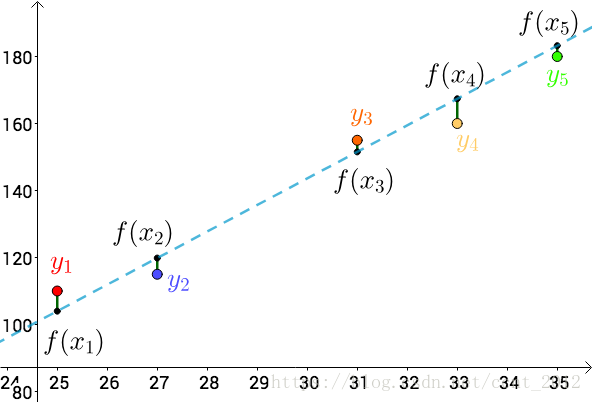
\includegraphics[width=0.9\textwidth]{least square.png}
    \textbf{Gram-Schmidt施密特正交化(4.3最后一题)}:先将A的列正交化(即将$x_i := x_i - 1/n\sum_{i=1}^{n}x_i$),然后便可以得到对角矩阵$A^T A$,这样求$\widehat{\bm{x}}$就很方便!
    \\
    \textbf{若A的列向量线性相关}\\
    涉及到奇异值分解SVD(7.4)\\
    因为A的列向量线性相关,若把b投影到A的列空间中,即改为$A \widehat{\boldsymbol{x}}=\boldsymbol{p}$,则此时会产生多个解,即有多条直线可以选,但是不知道哪条是最佳的!
    \\
    7.4中会利用A的伪逆"pseudoinverse"来选择一个最短解$\widehat{\bm{x}}$。\\
    若A的\textbf{列线性无关},它的伪逆是$L=\left(A^{\mathrm{T}} A\right)^{-1} A^{\mathrm{T}}$
    \\
    \textbf{拟合抛物线:}\\
    同样有m个点,$(t_{1},b_{1}), \dots, (t_{m},b_{m})$,利用$C+D t+E t^{2}$来拟合这些点!\\
    $$
    \begin{aligned} C+D t_{1}+E t_{1}^{2} &=b_{1} \\ \vdots & \\ C+D t_{m}+E t_{m}^{2} &=b_{m} \end{aligned}
    \begin{array}{l}{\text { is } A \boldsymbol{x}=\boldsymbol{b} \text { with }} \\ {\text { the } m \text { by } 3 \text { matrix }}\end{array}
    A=\left[\begin{array}{ccc}{1} & {t_{1}} & {t_{1}^{2}} \\ {\vdots} & {\vdots} & {\vdots} \\ {1} & {t_{m}} & {t_{m}^{2}}\end{array}\right]
    $$
    最接近的抛物线利用$\widehat{\boldsymbol{x}}=(C, D, E)$来满足正规方程组$A^{\mathrm{T}} A \widehat{\boldsymbol{x}}=A^{\mathrm{T}} \boldsymbol{b}$。即给出了最小二乘解(具有最小均方误差MSE)。
    \\
    \textbf{解耦uncouple}:指在线性方程组中只通过一个方程就可以解出一个变量的值。\\
    \textbf{耦合couple}:指单个方程里的多个变量只能通过整个方程组来解出。
    \\
    \textbf{递归最小二乘recursive least squares}:对旧均值增加一个新数据后,不用重新计算所有值之和再除以总数,$\{b_1,\dots, b_n\}+ b_{n+1},\quad \widehat{x}_{\mathrm{new}}=\widehat{x}_{\mathrm{old}}+\frac{1}{n+1}\left(b_{n+1}-\widehat{x}_{\mathrm{old}}\right)$
    \\
    \subsection{规范(标准)正交基和施密特正交化Orthonormal Bases and Gram-Schmidt}
    当$\boldsymbol{q}_{i}^{\mathrm{T}} \boldsymbol{q}_{j}=\left\{\begin{array}{ll}{0} & {\text { when } i \neq j \quad \text { orthogonal vectors }} \\ {1} & {\text { when } i=j \quad \text { (unit vectors: }\left\|\boldsymbol{q}_{i}\right\|=1 )}\end{array}\right.$
    \quad 向量$q_{1}, \dots, q_{n}$是规范正交的。\\
    若一个矩阵的列均为规范正交向量,则记为$\bm{Q}$,有$Q^{\mathrm{T}} Q=I$。 且若$Q$是\textbf{方阵},则称其为\textbf{正交矩阵orthogonal matrix},有$Q^{\mathrm{T}}=Q^{-1}$:\textbf{转置=逆}!
    \\
    \textbf{正交矩阵的作用:}
    \begin{itemize}
        \item \textbf{旋转Rotation} \quad (二维下)$Q=\left[\begin{array}{rr}{\cos \theta} & {-\sin \theta} \\ {\sin \theta} & {\cos \theta}\end{array}\right]$将向量旋转$\theta$度; \quad $Q^{\mathrm{T}}=Q^{-1}=\left[\begin{array}{rr}{\cos \theta} & {\sin \theta} \\ {-\sin \theta} & {\cos \theta}\end{array}\right]$将向量旋转$-\theta$度。
        \item \textbf{置换Permutation} \quad 每个置换矩阵都是正交矩阵,它的逆=转置!
        \item \textbf{反射Reflection} \quad 设$\bm{u}$是任意一个单位列向量,且$Q=I-2 u u^{\mathrm{T}}$,则有$Q^{\mathrm{T}}=I-2 u u^{\mathrm{T}}=Q$,$Q^{\mathrm{T}} Q=I-4 \boldsymbol{u u}^{\mathrm{T}}+4 \boldsymbol{u} \boldsymbol{u}^{\mathrm{T}} \boldsymbol{u} \boldsymbol{u}^{\mathrm{T}}=I$,反射矩阵可以将向量$u$转为$-u$。
    \end{itemize}
    一个向量乘上正交矩阵,它的\textbf{长度,角度都不改变}:$\|Q \boldsymbol{x}\|^{2}=(Q \boldsymbol{x})^{\mathrm{T}}(Q \boldsymbol{x})=\boldsymbol{x}^{\mathrm{T}} Q^{\mathrm{T}} Q \boldsymbol{x}=\boldsymbol{x}^{\mathrm{T}} I \boldsymbol{x}=\boldsymbol{x}^{\mathrm{T}} \boldsymbol{x}=\|\boldsymbol{x}\|^{2}$,即有$\|Q \boldsymbol{x}\|=\|\boldsymbol{x}\|$;也能使点积结果不变:$(Q \boldsymbol{x})^{\mathrm{T}}(Q \boldsymbol{y})=\boldsymbol{x}^{\mathrm{T}} Q^{\mathrm{T}} Q \boldsymbol{y}=\boldsymbol{x}^{\mathrm{T}} \boldsymbol{y}$
    \subsubsection{用规范正交基做投影,Q代替A}
    对于投影到子空间,通常利用$A^T A$,$A^T A$中的条目为$\boldsymbol{a}_{i}^{\mathrm{T}} \boldsymbol{a}_{j}$,即A的基的点积。\\
    \textbf{现假设A的基是规范正交的},则$A^T A$简化为$Q^T Q=I$(解耦了),且:
    \begin{itemize}
        \item $Q^T Q\widehat{\boldsymbol{x}}=Q^{\mathrm{T}} \boldsymbol{b} \rightarrow \widehat{\boldsymbol{x}}=Q^{\mathrm{T}} \boldsymbol{b}$
        \item $\bm{p}=Q \widehat{\bm{x}} = Q Q^{\mathrm{T}} \bm{b}$
        \item $P=Q(Q^T Q)^{-1}Q^{\mathrm{T}} \rightarrow P=Q Q^T$
    \end{itemize}
    $\boldsymbol{p}=Q Q^{\mathrm{T}} \bm{b}=\left[\begin{array}{lll}{|} & {} & { |} \\ {\bm{q}_{1}} & {\cdots} & {\bm{q}_{n}} \\ { |} & {} & { |}\end{array}\right]\left[\begin{array}{c}{\bm{q}_{1}^{\mathrm{T}} \bm{b}} \\ {\vdots} \\ {\bm{q}_{n}^{\mathrm{T}} \bm{b}}\end{array}\right]=\boldsymbol{q}_{1}\left(\boldsymbol{q}_{1}^{\mathrm{T}} \boldsymbol{b}\right)+\cdots+\boldsymbol{q}_{n}\left(\boldsymbol{q}_{n}^{\mathrm{T}} \boldsymbol{b}\right)$
    \\
    当Q为方阵时,列空间便为整个空间,$Q^{\mathrm{T}}=Q^{-1}$,$\boldsymbol{x}=Q^{-1} \boldsymbol{b}$,最小二乘解是精确的,$\bm{b}$在整个空间上的投影是它自己,$P=Q Q^{\mathrm{T}}=I$。
    \\
    $\boldsymbol{p}=\boldsymbol{b}=Q Q^{\mathrm{T}} \bm{b}=\bm{q}_{1}\left(\bm{q}_{1}^{\mathrm{T}} \bm{b}\right)+\bm{q}_{2}\left(\bm{q}_{2}^{\mathrm{T}} \bm{b}\right)+\cdots+\bm{q}_{n}\left(\bm{q}_{n}^{\mathrm{T}} \bm{b}\right)$,这说明了每个$\bm{b}$是沿着Q的基方向的每个$\bm{b}$的分量之和!$\widehat{\bm{x}}_i = \bm{q}^T_{i} \bm{b}, \quad \bm{q}_i \widehat{\bm{x}}_i$\textbf{是向量b在第i个基上的投影!故每个基上的投影加起来便是原向量b!(用于QR分解的理解!)}
    \\
    $Q Q^{\mathrm{T}}=I$是傅里叶变换基础,这些变换将向量或者函数分解成垂直片断,再通过上式利用逆变换将这些片段放到一起组成向量或者函数f。

    \subsubsection{施密特正交化}
    思想:新向量减去它在已有的正交向量上的投影向量,即求误差$e$,这就是新的正交向量!最后对每个正交向量除以自己的长度,进行归一化!
    \subsubsection{$A_{m\times n}=Q_{m\times m}R_{m\times n}$分解}
    将上述的A与Q(规范正交矩阵)用R(上三角矩阵)联系起来,\textbf{A--->施密特正交化--->Q},每一步$\boldsymbol{a}_{1}, \dots, \boldsymbol{a}_{k}$都是$q_{1}, \ldots, q_{k}$的线性组合,后面的$\bm{q}_{k+1}...$均不涉及。正交化过程中用到的转换矩阵便是$T,R=T^{-1}$。
    \\
    $A=Q R=$
    $\left[\begin{array}{lll}{\bm{a}} & {\bm{b}} & {\bm{c}}\end{array}\right]=\left[\begin{array}{lll}{\bm{q}_{1}} & {\bm{q}_{2}} & {\bm{q}_{3}}\end{array}\right]\left[\begin{array}{ccc}{\bm{q}_{1}^{T} \bm{a}} & {\bm{q}_{1}^{T} \bm{b}} & {\bm{q}_{1}^{T} \bm{c}} \\ {} & {\bm{q}_{2}^{T} \bm{b}} & {\bm{q}_{2}^{T} \bm{c}} \\ {} & {} & {\bm{q}_{3}^{T} \bm{c}}\end{array}\right]$
    \\
    简而言之,$A=Q R$就是Gram-Schmidt,左乘一个$Q^T$得:$\boldsymbol{R}=\boldsymbol{Q}^{\mathrm{T}} \boldsymbol{A}$,其中$R$为上三角矩阵!(因为$Q^T Q = I$)
    
    \subsubsection{Problem set}
    4. (a) Any $Q_{m\times n}$ with $n<m$ has $Q Q^{\mathrm{T}} \neq I$,如$Q=\left[\begin{array}{ll}{1} & {0} \\ {0} & {1} \\ {0} & {0}\end{array}\right], Q Q^{\mathrm{T}}=\left[\begin{array}{ccc}{1} & {0} & {0} \\ {0} & {1} & {0} \\ {0} & {0} & {0}\end{array}\right] \neq I$
    \\
    若A能QR分解,则$A^{\mathrm{T}} A=R^{\mathrm{T}} R$下三角乘上三角。

    \section{行列式(方阵) Determinants}
    \subsection{性质properties}
    \begin{itemize}
        \item A可逆,则$\bm{det}(A) \neq 0$
        \item $det(A^{-1})$ = 1$/(\operatorname{det} A)$
    \end{itemize}
    反对称矩阵skew-symmetric matrix $A^{\mathrm{T}}=-A$
    \subsection{排列和代数余子式Permutations and Cofactors}
    \textbf{求行列式的三种方法}
    \begin{itemize}
        \item 消元法 Pivot formula 将矩阵化为三角矩阵,即进行LU分解。
        \item 逆序数法 Big formula 每个$n\times n$矩阵的行列式都有$n!$个项,每个项里的元素均为不同行不同列的元素,元素的行列不能有重合!
        \item 代数余子式法 Cofactors $\operatorname{det} A=a_{11}\left(a_{22} a_{33}-a_{23} a_{32}\right)+a_{12}\left(a_{23} a_{31}-a_{21} a_{33}\right)+a_{13}\left(a_{21} a_{32}-a_{22} a_{31}\right)$,括号里的便是代数余子式。$\operatorname{det} A=a_{i 1} C_{i 1}+a_{i 2} C_{i 2}+\cdots+a_{i n} C_{i n}$,$C_{i j}=(-1)^{i+j} \operatorname{det} M_{i j}$。
    \end{itemize}

    \subsection{Cramer's Rule, Inverses, and Volumes}
    Cramer's Rule(可逆方阵):$\left[\begin{array}{l}{A} \\ {}\end{array}\right]\left[\begin{array}{lll}{x_{1}} & {0} & {0} \\ {x_{2}} & {1} & {0} \\ {x_{3}} & {0} & {1}\end{array}\right]=\left[\begin{array}{lll}{b_{1}} & {a_{12}} & {a_{13}} \\ {b_{2}} & {a_{22}} & {a_{23}} \\ {b_{3}} & {a_{32}} & {a_{33}}\end{array}\right]=B_{1}$
    \\
    $(\operatorname{det} A)\left(x_{1}\right)=\operatorname{det} B_{1} \quad$ or $\quad x_{1}=\frac{\operatorname{det} B_{1}}{\operatorname{det} A}$,$x_2,x_3$同理\\
    故若$det(A)\neq 0, A \bm{x}=\bm{b}$则有:$x_{1}=\frac{\operatorname{det} B_{1}}{\operatorname{det} A} \quad x_{2}=\frac{\operatorname{det} B_{2}}{\operatorname{det} A} \quad \ldots \quad x_{n}=\frac{\operatorname{det} B_{n}}{\operatorname{det} A}$
    \\
    $A^{-1}$包含$A$的代数余子式,同样利用cramer法则解决$AA^{-1}=I$:\\
    \\
    过程:$AA^{-1}=A\left[\begin{array}{lll} \bm{col1} & \bm{col2} & \bm{col3} \end{array}\right] = \left[\begin{array}{lll}
    1 & 0 & 0 \\0 & 1 & 0 \\0 & 0 & 1
    \end{array}\right]$,将其中每一个等式单独拿出来利用Cramer法则进行计算,例如$A \boldsymbol{x}=(1,0,0)$\\
    $\left|\begin{array}{lll}{1} & {a_{12}} & {a_{13}} \\ {0} & {a_{22}} & {a_{23}} \\ {0} & {a_{32}} & {a_{33}}\end{array}\right| \quad\left|\begin{array}{lll}{a_{11}} & {1} & {a_{13}} \\ {a_{21}} & {0} & {a_{23}} \\ {a_{31}} & {0} & {a_{33}}\end{array}\right| \quad\left|\begin{array}{lll}{a_{11}} & {a_{12}} & {1} \\ {a_{21}} & {a_{22}} & {0} \\ {a_{31}} & {a_{32}} & {0}\end{array}\right|$
    \\
    所以每个$|B_{j}|$都是$A$的代数余子式! 故有:$\left(A^{-1}\right)_{i j}=\frac{C_{j i}}{\operatorname{det} A} \quad$ and $\quad A^{-1}=\frac{C^{\mathrm{T}}}{\operatorname{det} A}$
    \\
    \textbf{二阶行列式是平行四边形的面积,是三角形面积的一半!} \\
    通过面积$s=\bm{ab}\sin \theta$证明。
    \\
    \textbf{矩阵的行列式其实是该矩阵变换下的图形面积或体积的伸缩因子。}(Jacobian matrix 雅可比矩阵) \\
    \textbf{叉乘 Cross Product}\\
    叉乘只用于三维空间中,结果为向量:$\bm{u}=\left(u_{1}, u_{2}, u_{3}\right)$ $\bm{v}=\left(v_{1}, v_{2}, v_{3}\right)$
    \\
    $\bm{u} \times \bm{v}=\left|\begin{array}{ccc}\bm{i} & \bm{j} & \bm{k} \\ {u_{1}} & {u_{2}} & {u_{3}} \\ {v_{1}} & {v_{2}} & {v_{3}}\end{array}\right|=\left(u_{2} v_{3}-u_{3} v_{2}\right) \bm{i}+\left(u_{3} v_{1}-u_{1} v_{3}\right) \bm{j}+\left(u_{1} v_{2}-u_{2} v_{1}\right) \bm{k}$
    \\
    向量$\bm{u} \times \bm{v}$垂直于$\bm{u}$和$\bm{v}$。此外,$|\bm{u} \times \bm{v}|=\|\boldsymbol{u}\|\|\boldsymbol{v}\||\sin \theta|$在数值上等于由向量$\bm{u}$和向量$\bm{v}$构成的平行四边形的面积。
    \\
    \textbf{三重积(混合积)triple product} \\
    混合积是一个标量scalar,且它是这三个向量构成的体积!\\
    $(\boldsymbol{u} \times \boldsymbol{v}) \cdot \boldsymbol{w}=\left|\begin{array}{lll}{w_{1}} & {w_{2}} & {w_{3}} \\ {u_{1}} & {u_{2}} & {u_{3}} \\ {v_{1}} & {v_{2}} & {v_{3}}\end{array}\right|=\left|\begin{array}{ccc}{u_{1}} & {u_{2}} & {u_{3}} \\ {v_{1}} & {v_{2}} & {v_{3}} \\ {w_{1}} & {w_{2}} & {w_{3}}\end{array}\right|$
    \\
    当$\bm{u,v,w}$均位于同一平面时,混合积为零。

    \section{特征值和特征向量Eigenvalues and Eigenvectors}
    \subsection{特征值 Eigenvalues}
    $A \boldsymbol{x}=\lambda \boldsymbol{x}$, 其中$\bm{x}$是特征向量,$\lambda$是特征值(可以为0,说明特征向量处于零空间中)!
    \\
    特征向量乘上A不改变方向,其他向量会改变方向。但是\textbf{其他向量可以用特征向量的线性组合来表示!}
    \\
    这里引入\textbf{马尔科夫矩阵Markov matrix}:它的每一列相加为1,最大特征值为1,对应特征向量处于一种稳定状态(当A乘上$A^{k}$时,A的所有列都会达到的一个稳定状态)\\
    $A^{99}\left[\begin{array}{l}{.8} \\ {.2}\end{array}\right] \quad$ is really $\quad \boldsymbol{x}_{1}+(.2)\left(\frac{1}{2}\right)^{99} \boldsymbol{x}_{2}=\left[\begin{array}{l}{.6} \\ {.4}\end{array}\right]+\left[\begin{array}{l}{\text { very }} \\ {\text { small }} \\ {\text { vector }}\end{array}\right]$(这里将A的其中一列乘上$A^{99}$)
    \subsubsection{特征值方程}
    $A \boldsymbol{x}=\lambda \boldsymbol{x} \rightarrow (A-\lambda I) \bm{x}=\bm{0}$,也就是说特征向量$\bm{x}$构成了零空间,说明方程组必有非零解,即行列式为0。
    \\
    $\lambda$为特征值当且仅当$(A-\lambda I)$是奇异的(不可逆),即$\operatorname{det}(A-\lambda I)=0$。
    \\
    特征多项式(characteristic polynomial) $\operatorname{det}(A-\lambda I)$仅包含$\lambda$,当矩阵A是$n \times n$时,有n个特征值(可能重复)。
    \\
    计算过程省略。。。
    \subsubsection{行列式和迹 determinant and trace}
    \begin{itemize}
        \item $det(A)=\lambda_{1}\lambda_{2}\dots\lambda_{n}$
        \item $trace(A) = \lambda_{1}+\lambda_{2}+\cdots+\lambda_{n}=a_{11}+a_{22}+\cdots+a_{n n}$
        \item 三角阵对角线上的元素即为它的特征值!
    \end{itemize}
    \textbf{上述前两条证明需要用到推广韦达定理,行列式展开式,具体证明见chrome收藏:mit线性代数}
    \subsubsection{AB和A+B的特征值}
    \textbf{错误证明}:$A B \boldsymbol{x}=A \beta \boldsymbol{x}=\beta A \boldsymbol{x}=\beta \lambda \boldsymbol{x}$,这是\textbf{因为特征向量$\bm{x}$不一定同时是A和B的特征向量!}
    \\
    \textbf{同理,A+B的特征值也不一定是$\lambda + \beta$}。上述情况只有在$\bm{x}$同时为A,B的特征向量时才成立!
    \\
    当且仅当$A B=B A$时,A,B同时共享相同的n个特征向量!\\
    \textbf{对称矩阵的特征值为实数,反对称矩阵的特征值为虚数!}
    \subsection{对角化, 相似}
    \subsubsection{对角化Diagonalization}
    若矩阵A有n个线性无关的特征向量,将它们放入特征向量矩阵$X$中,则有$X^{-1} A X=\Lambda=\left[\begin{array}{ccc}{\lambda_{1}} & {} & {} \\ {} & {\ddots} & {} \\ {} & {} & {\lambda_{n}}\end{array}\right]$,大写lambda $\Lambda$的对角线是特征值!
    \\
    解释$A X=X \Lambda$:$A X=A\Bigg[\begin{array}{lll}{x_{1}} & {\cdots} & {x_{n}}\end{array}\Bigg]=\Bigg[\begin{array}{lll}{\lambda_{1} x_{1}} & {\cdots} & {\lambda_{n} x_{n}}\end{array}\Bigg]$
    $=\Bigg[\begin{array}{ccc}{x_{1}} & {\cdots} & {x_{n}}\end{array}\Bigg]\Bigg[\begin{array}{ccc}{\lambda_{1}} & {} \\ {} & {\ddots} & {} \\ {} & {} & {\lambda_{n}}\end{array}\Bigg]=X \Lambda$
    \\
    故$A X=X \Lambda \rightarrow X^{-1} A X=\Lambda \quad$ or $\quad A=X \Lambda X^{-1}$。$A$和$\Lambda$的特征值相同,特征向量不同!
    \\
    $A^{k}=\left(X \Lambda X^{-1}\right)\left(X \Lambda X^{-1}\right) \ldots\left(X \Lambda X^{-1}\right)=X \Lambda^{k} X^{-1}$
    \\
    只有当\textbf{A有n个线性无关的特征向量时,才能对角化}。P306(316)利用构造线性组合证明了不同特征值对应的特征向量线性无关!

    \subsubsection{相似矩阵:相同特征值}
    假设$\Lambda$不变,改变特征矩阵$X$,这样会得到所有能相似对角化成$\Lambda$。\\
    \textbf{相似定义:存在可逆矩阵$B$,若$A=B C B^{-1}$,则称A与C相似(C不一定是对角阵)。}\\
    事实上,若A,C\textbf{相似},则它们一定\textbf{有相同的特征值}!\\
    \textbf{Proof:}假设$C \boldsymbol{x}=\lambda \boldsymbol{x}$,则对于$A=B C B^{-1}$可以找到特征向量$B \boldsymbol{x}$使得:$\left(B C B^{-1}\right)(B \boldsymbol{x})=B C \boldsymbol{x}=B \lambda \boldsymbol{x}=\lambda(B \boldsymbol{x})$,即$A(B\bm{x})=\lambda (B\bm{x})$。

    \subsubsection{若尔当型标准型 Jordan Form}
    Jordan Block: $J_{i}=\left(\begin{array}{cccccc}{\lambda_{i}} & {1} & {} & {} & {} \\ {} & {\lambda_{i}} & {1} & {} & {} &{} \\ {} & {} & {\lambda_{i}} & {\ddots} & {}&{} \\ {} & {} & {} & {\ddots} & {1}&{} \\ {} & {} & {} &{} & {\lambda_{i}} & {1} \\ {}&{} & {} & {} & {} & {\lambda_{i}}\end{array}\right)_{r_{i}\times r_{i}}$,对角线上是重复的特征值,每个特征值上面有1,其余元素都是0.
    \\
    对于任一n阶复数矩阵A,都与一个若尔当型矩阵J相似,其中$J=\left[\begin{array}{cccc} J_{1} & & & \\ &J_{2} & & \\ & &  \ddots &\\  & & & J_{r_{i}}
    \end{array}\right]$,且$1+2+\cdots +r_{i}=n$,每一个若尔当块对应一个特征向量,所以A的若尔当块数=特征向量数。(若有n个特征向量,n个分块,即$r_{i}=n$,则说明矩阵A可以对角化即$J=\Lambda$)
    \\
    \textbf{在不计Jordan块次序的前提下,A的Jordan标准型矩阵是唯一确定的}。
    \\
    Jordan Form 矩阵是指最接近对角阵但是又无法对角化的矩阵!比如$\begin{bmatrix}4 & 1 \\ 0 & 4\end{bmatrix}$ 它不可能对角化(因为$\Lambda = 4I$利用谱定理得到的总是$4I$)。\\
    同样有两个不能对角化的矩阵,它们有相同特征值0,相同数量的特征向量:$\left[\begin{array}{lll|l}{0} & {1} & {0} & {0} \\ {0} & {0} & {0} & {0}\\{0}&{0} & {0} & {1} \\ \hline {0}&{0} & {0} & {0}\end{array}\right]$和$\left[\begin{array}{ll|ll}{0} & {1} & {0} & {0} \\ {0} & {0} & {1} & {0} \\ \hline {0}&{0} & {0} & {0} \\{0}&{0} & {0} & {0}\end{array}\right]$,\textbf{尽管它们特征值相同,但是由于它们的Jordan block分块不同,所以不相似!}


    \subsubsection{Fibonacci Numbers}
    斐波那契数列 $\quad 0,1,1,2,3,5,8,13, \ldots \quad$ 有递推式 $\quad F_{k+2}=F_{k+1}+F_{k}$,可以利用矩阵方程$\mathbf{u}_{k+1}=A \boldsymbol{u}_{k}$来快速计算。
    \\
    设$\bm{u}_{k}=\left[\begin{array}{c}{F_{k+1}} \\ {F_{k}}\end{array}\right] $\quad 递推式 $\begin{aligned} F_{k+2} &=F_{k+1}+F_{k} \\ F_{k+1} &=F_{k+1} \end{aligned}$ 可以表示为 $\bm{u}_{k+1}=\left[\begin{array}{cc}{1} & {1} \\ {1} & {0}\end{array}\right] \bm{u}_{k}$
    \\
    所以每求一步新的斐波那契数就乘上一个矩阵$A=\left[\begin{array}{ll}{1} & {1} \\ {1} & {0}\end{array}\right]$,\textbf{差分方程}$\bm{u}_{100} = A^{100} \bm{u}_0$ 即
    $u_{0}=\left[\begin{array}{l}{1} \\ {0}\end{array}\right], \quad u_{1}=\left[\begin{array}{l}{1} \\ {1}\end{array}\right], \quad u_{2}=\left[\begin{array}{l}{2} \\ {1}\end{array}\right], \quad u_{3}=\left[\begin{array}{l}{3} \\ {2}\end{array}\right], \quad \ldots, \quad u_{100}=\left[\begin{array}{l}{F_{101}} \\ {F_{100}}\end{array}\right]$
    \\
    为了简化矩阵乘法,使其能快速求解,\textbf{利用A的特征值:}\\
    $A-\lambda I=\left[\begin{array}{cc}{1-\lambda} & {1} \\ {1} & {-\lambda}\end{array}\right] \rightarrow det(A-\lambda I)=\lambda^{2}-\lambda-1=0 \rightarrow$\\
    $Eigenvalues: \lambda_1 = \frac{1+\sqrt{5}}{2} \approx 1.618 \quad \lambda_2 = \frac{1-\sqrt{5}}{2} \approx -0.618$\\
    $Eigenvectors: \bm{x}_1 = (\lambda_1,1)\quad \bm{x}_2 = (\lambda_2,1)$
    然后将$\bm{u}_0$\textbf{表示为两个特征向量的线性组合}:$\bm{u}_0 =\frac{\bm{x}_1-\bm{x}_2}{\lambda_1 - \lambda_2} \rightarrow \left[\begin{array}{c} 1 \\ 0 \end{array}\right]= \frac{1}{\lambda_1 - \lambda_2}\left(\left[\begin{array}{c} \lambda_1 \\ 1 \end{array}\right]- \left[\begin{array}{c} \lambda_2 \\ 1 \end{array}\right]\right)$
    \\
    再计算$\bm{u}_{100} = A^{100} \bm{u}_0$,即将$\bm{u}_0$乘上$A^{100}$,就有:$\bm{u}_{100}= \frac{(\lambda_1)^{100}\bm{x}_1 - (\lambda_2)^{100}\bm{x}_2}{\lambda_1 - \lambda_2}$。而且$\lambda_2^{100} \approx 0$,所以第100个数为$\frac{\lambda_1^{100} - \lambda_2^{100}}{\lambda_1 - \lambda_2}$近似于$\frac{1}{\sqrt{5}}\left(\frac{1+\sqrt{5}}{2}\right)^{100}$。
    \\
    每个$F_k$都是整数,且比例$F_101 / F_100$是非常接近$\frac{1+\sqrt{5}}{2}$的。

    \subsubsection{矩阵的幂}
    矩阵的对角化分解非常适合用来计算矩阵的幂,例如上一小节的差分方程:$\bm{u}_{100} = A^{100} \bm{u}_0$中,$A^{k}\bm{u}_0=(X\Lambda X^{-1})\cdots (X\Lambda X^{-1})\bm{u}_0=(X\Lambda^{k} X^{-1})\bm{u}_0$。
    \\
    下面分步解释特征值在其中是如何起作用的(详细说明P310(320)):
    \begin{enumerate}
        \item 写成线性组合用特征向量表出$\bm{u}_0 = c_1\bm{x}_1 + \cdots + c_n\bm{x}_n, \quad  \bm{u}_0= X \bm{c}_{n\times 1} \quad \bm{c}_{n\times 1}= X^{-1}\bm{u}_0$
        \item 每个特征向量$\bm{x}_i$乘上$(\lambda_i)^k$,即有$\Lambda^k X^{-1}\bm{u}_0$
        \item 在乘上$X$得到$c_i (\lambda_i)^k\bm{x}_i$,全部加起来便是$X\Lambda^{k} X^{-1}\bm{u}_0$
    \end{enumerate}
    所以最终解的形式:$\bm{u}_k =c_1 (\lambda_1)^k\bm{x}_1+\cdots +c_n (\lambda_n)^k\bm{x}_n =\sum{ c_i (\lambda_i)^k\bm{x}_i}$。

    \subsubsection{不可对角化的矩阵Nondiagonalizable Matrices}
    也就是有重复的特征值$\lambda$,但是对应$\lambda$的\textbf{特征向量个数GM不等于特征值重复的次数AM!}

    欧拉公式Euler's formula: $e^{i\theta} = cos\theta + isin\theta$
    \begin{itemize}
        \item A,B均为方阵时,AB,BA有相同特征值值
        \item 当$A_{m\times n}, B_{n\times m}$时,AB,BA有相同的非零特征值
    \end{itemize}
    证明见百度(利用特征值公式)~

    \subsection{微分方程组Systems of Differential Equations}
    A的相似对角化不仅适用于计算$A^k$,也适用于计算微分方程$d\bm{u}/dt = A\bm{u}$。此章节主要是:\textbf{将线性常系数微分方程转换为线性代数!}
    \\
    \textbf{普通微分方程}$\frac{du}{dt} = u \rightarrow u(t)=\bm{Ce^t}, \quad \frac{du}{dt} = \lambda u \rightarrow u(t)=\bm{Ce^{\lambda t}}$,当time t=0时,有$u(0)=c$,说明了解的系数$\bm{C}$。
    \\
    但以上只是从一个方程出发,\textbf{若有多个微分方程联立共同确定几个具有同一自变量的函数,这构成了微分方程组(耦合),它的解是关于共同自变量的函数。未知数(函数)可以写成向量},从给定的初始条件$\bm{u(0)}$开始。
    \\
    \textbf{例如}:$\left\{\begin{array}{l} \frac{du_1}{dt}=-u_1+2u_2 \\ \frac{du_2}{dt}=u_1-2u_2 \end{array}\right.$ 写成向量形式:$\dfrac{d}{dt} \begin{bmatrix}u_1 \\ u_2 \end{bmatrix}=\begin{bmatrix}-1 & 2 \\ 1 & -2 \end{bmatrix}\begin{bmatrix}u_1 \\ u_2 \end{bmatrix} \rightarrow \dfrac{d\bm{u}}{dt}=A\bm{u}$
    \\
    即$\frac{d\bm{u}}{dt}= \bm{u}$从向量$\bm{u}(0)=\begin{bmatrix} u_{1}(0) \\ \cdots \\ u_{n}(0) \end{bmatrix}$开始!
    利用$A \boldsymbol{x}=\lambda \boldsymbol{x}$找到纯指数解$e^{\lambda t} \bm{x}$。

    \subsubsection{$d \boldsymbol{u} / d t=A \boldsymbol{u}$的解}
    纯指数解为$\boldsymbol{u}(t)=e^{\lambda t} \boldsymbol{x}$,其中$\lambda$是A的特征值,$\bm{x}$是A的特征向量。$\frac{d \boldsymbol{u}}{d t}=\lambda e^{\lambda t} \boldsymbol{x}$与$A \boldsymbol{u}=A e^{\lambda t} \boldsymbol{x}$一致。
    \\
    求解过程:
    \begin{enumerate}
        \item 将初始状态$\boldsymbol{u}(0)$表示为A特征向量的线性组合$c_{1} \boldsymbol{x}_{1}+\cdots+c_{n} \boldsymbol{x}_{n}$(需要A能相似对角化,即有n个线性无关的特征向量)
        \item 对每个特征向量$\boldsymbol{x}_{i}$乘上对应的$e^{\lambda_{i} t}$
        \item 所以微分方程组$\dfrac{d \bm{u}}{d t}=A \bm{u}$的通解为:$\bm{u}(t)=c_{1} e^{\lambda_{1} t} \bm{x}_{1}+\cdots+c_{n} e^{\lambda_{n} t} \bm{x}_{n}$
    \end{enumerate}
    若A有重复特征值且GM!=AM,即特征向量个数不等于重复数,则通解中会包含$t e^{\lambda t} \boldsymbol{x}$。

    \subsubsection{二阶微分方程的解}
    高数中:$m \frac{d^{2} y}{d t^{2}}+b \frac{d y}{d t}+k y=0 \quad$ becomes $\quad\left(m \lambda^{2}+b \lambda+k\right) e^{\lambda t}=0$,且利用$y=e^{\lambda t}$来解微分方程,即$y_{1}=e^{\lambda_{1} t}$ and $y_{2}=e^{\lambda_{2} t}$。($\lambda_1 \lambda_2 $是特征方程的两个根!)
    \\
    线代中:利用特征值和特征矩阵来解方程,先对该二阶微分方程$m \frac{d^{2} y}{d t^{2}}+b \frac{d y}{d t}+k y=0$构造方程组,设$m=1$(不设也没关系),$\boldsymbol{u}=\left(y, y^{\prime}\right)$\textbf{降阶处理}:
    \begin{enumerate}
        \item $\left\{\begin{array}{l}{d y / d t=y^{\prime}} \\ {d y^{\prime} / d t=-k y-b y^{\prime}}\end{array}\right. \rightarrow \dfrac{d}{d t}\left[\begin{array}{l}{y} \\ {y^{\prime}}\end{array}\right]=\left[\begin{array}{rr}{\mathbf{0}} & {\mathbf{1}} \\ {-\boldsymbol{k}} & {-\boldsymbol{b}}\end{array}\right]\left[\begin{array}{l}{y} \\ {y^{\prime}}\end{array}\right]=A \boldsymbol{u}$,第一个式子是不必要的(为了构建矩阵),第二个式子把$y^{\prime \prime}$连接到$y^{\prime}$和$y$,所以宏观看来这是$\boldsymbol{u}^{\prime}$ 转为 $\boldsymbol{u}$。
        \item $A-\lambda I=\left[\begin{array}{cc}{-\lambda} & {1} \\ {-k} & {-b-\lambda}\end{array}\right]$有行列式$\lambda^{2}+b \lambda+k=0$,这与高数中的一致!求出特征值$\lambda_1, \lambda_2$ 特征向量$\boldsymbol{x}_{1}=\left[\begin{array}{l}{1} \\ {\lambda_{1}}\end{array}\right]$\quad $\boldsymbol{x}_{2}=\left[\begin{array}{c}{1} \\ {\lambda_{2}}\end{array}\right]$
        \item 得到方程组通解:$u(t)=c_{1} e^{\lambda_{1} t}\left[\begin{array}{c}{1} \\ {\lambda_{1}}\end{array}\right]+c_{2} e^{\lambda_{2} t}\left[\begin{array}{c}{1} \\ {\lambda_{2}}\end{array}\right]$
        \item 方程组通解第一个元素:$y=c_{1} e^{\lambda_{1} t}+c_{2} e^{\lambda_{2} t}$就是该二阶微分方程的通解。
        \item 第二个元素便是$d y / d t$。
    \end{enumerate}
    \textbf{求解3阶...n阶微分方程同理, 仿照上述方法构造矩阵即可。}

    \subsubsection{2×2矩阵的稳定性}
    微分方程$d \boldsymbol{u} / d t=A \boldsymbol{u}$的通解$\bm{u}(t)$,当$t \rightarrow \infty$时,通解是趋于0?
    通解$\bm{u}(t)$是从$e^{\lambda t} \boldsymbol{x}$得来的,所以:
    \begin{itemize}
        \item 若特征值$\lambda$是实数,则$\lambda < 0$才有$e^{\lambda t} \rightarrow 0$
        \item 若特征值$\lambda$是复数,则$\lambda=r+i s$的实部$r <0$才有$e^{\lambda t} \rightarrow 0$。\\注意:$e^{\lambda t}$分解成$e^{r t} e^{i s t}$,因为$e^{i s t}=\cos s t+i \sin s t$(欧拉公式)有$\quad\left|e^{i s t}\right|^{2}=\cos ^{2} s t+\sin ^{2} s t=1$,所以$e^{i s t}$固定为1,不影响解的值!
    \end{itemize}
    对于2×2矩阵来说,A所有特征值实部均为负数方程的解才会趋于稳定,可以用矩阵的迹trace(A)<0和行列式det(A)>0来判断。

    \subsubsection{解耦与矩阵指数 uncouple and exponential of a matrix}
    一般来说,微分方程组中各个同自变量的函数(即未知数)是耦合的,利用A的特征值和特征向量进行\textbf{对角化}就可以进行\textbf{解耦}。
    \\
    首先定义\textbf{矩阵指数$e^{A t}$}, 把指数展开成幂级数的方式,\textbf{当指数是矩阵时也一样}!(特征向量矩阵$X$,且$A=X\Lambda X^{-1}$):
    \begin{enumerate}
        \item 幂级数公式:$e^{\mathrm{x}}=1+\mathrm{x}+\dfrac{x^{2}}{2}+\dfrac{x^{3}}{6}+ \dots +\dfrac{x^{n}}{\mathrm{n} !}\cdots$ \quad (收敛域为全体实数)
        \item 扩展到矩阵计算中,I代替1,矩阵代替x :\\
        $e^{A t}=I+A t+\dfrac{(A t)^{2}}{2}+\dfrac{(A t)^{3}}{6}+\dots \cdots \cdots+\dfrac{(A t)^{n}}{n !}+\cdots \cdots$
        \item 对角化A:$e^{A t}=I+X \Lambda X^{-1} t+\frac{1}{2}\left(X \Lambda X^{-1} t\right)\left(X \Lambda X^{-1} t\right)+\cdots$\\
        $=X\left[I+\Lambda t+\frac{1}{2}(\Lambda t)^{2}+\cdots\right] X^{-1}$
        \item 对比e的幂级数展开式可知:$e^{A t}=X e^{\Lambda t} X^{-1}$
    \end{enumerate}
    \textbf{矩阵分析中有证明矩阵的泰勒展开式与函数的泰勒展开式的形式一样!}\\
    $\Lambda=\left[\begin{array}{ccc}{\lambda_{1}} & {} & {} \\ {} & {\ddots} & {} \\ {} & {} & {\lambda_{n}}\end{array}\right]$ \quad
    $e^{\Lambda t} = \left[\begin{array}{ccc}{e^{\lambda_{1} t}} & {} & {} \\ {} & {\ddots} & {} \\ {} & {} & {e^{\lambda_{n} t}}\end{array}\right]$
    \\
    \textbf{解耦:}在之前的$\dfrac{d\bm{u}}{dt}=A\bm{u}$中,有$u_1, u_2$耦合,
    \begin{enumerate}
        \item 设$\bm{u}=X\bm{v}$, $\dfrac{{d} \bm{u}}{dt}={S} \dfrac{{d} \bm{v}}{{dt}}=A\bm{u}=AX\bm{v}$
        \item 提取出${S} \dfrac{{d} \bm{v}}{{dt}}=AX\bm{v}$,左右两边同时乘上$X^{-1}$得到:\\
        $\dfrac{{d} \bm{v}}{{dt}}=X^{-1}AX\bm{v} = \Lambda v$
        \item 由此得到关于$\bm{v}$的对角化方程组,不耦合---$\dfrac{\mathrm{d} v_{1}}{\mathrm{dt}}=\lambda_{1} v_{1}, \dfrac{\mathrm{d} v_{2}}{\mathrm{dt}}=\lambda_{2} v_{2}$
        \item 最终有:$\bm{v}(\mathrm{t})=e^{\Lambda \mathrm{t}} \bm{v}(0)$且$\bm{u}(t)=e^{A t} \bm{u}(0)=\mathrm{Xe}^{\Lambda \mathrm{t}} X^{-1} \bm{u}(0)$
    \end{enumerate}
    $e^{A t} \bm{u}(0)=X e^{\Lambda t} X^{-1} \bm{u}(0)=\left[\begin{array}{ccc}{\bm{x}_{1}} & {\cdots} & {\bm{x}_{n}}\end{array}\right]\left[\begin{array}{ccc}{e^{\lambda_{1} t}} & {} & {} \\ {} & {\ddots} & {} \\ {} & {} & {e^{\lambda_{n} t}}\end{array}\right]\left[\begin{array}{c}{c_{1}} \\ {\vdots} \\ {c_{n}}\end{array}\right]$
    \\
    $\boldsymbol{u}(0)=c_{1} \boldsymbol{x}_{1}+\cdots+c_{n} \boldsymbol{x}_{n}=X \boldsymbol{c}$,\quad
    故它与之前提到的解微分方程组三步解法得到的\textbf{通解}$\boldsymbol{u}(t)=\boldsymbol{c}_{1} e^{\boldsymbol{\lambda}_{1} \boldsymbol{t}} \boldsymbol{x}_{1}+\cdots+\boldsymbol{c}_{\boldsymbol{n}} \boldsymbol{e}^{\boldsymbol{\lambda}_{\boldsymbol{n}} \boldsymbol{t}} \boldsymbol{x}_{\boldsymbol{n}}$\textbf{是一样的}!
    \\
    \textbf{{P327(337) example4}}解释了\textbf{为什么在解一个二阶微分方程式会出现: $e^{t}$ 和 $t e^{t}$},其核心在于A有重复特征值且特征向量数目不够,则$e^{A t}=e^{I t} e^{(A-I) t}=e^{t}[I+(A-I) t]$($e^{(A-I) t}$的幂级数展开式是收敛的,因为$(A-I)^{2}$是零矩阵)\\
    $\left[\begin{array}{l}{y} \\ {y^{\prime}}\end{array}\right]=e^{t}\left[I+\left[\begin{array}{cc}{-1} & {1} \\ {-1} & {1}\end{array}\right] t\right]\left[\begin{array}{c}{y(0)} \\ {y^{\prime}(0)}\end{array}\right]$, $y(t)=e^{t} y(0)-t e^{t} y(0)+t e^{t} y^{\prime}(0)$
    \\
    \textbf{Problem Set 26证明了$e^{At}$为什么是可逆的!(所有特征值$e^{\lambda t}>0$)}\\

    \subsection{对称阵 symmetric matrices}
    key fact:
    \begin{itemize}
        \item 一个实对称阵只有实特征值
        \item 特征向量可以选择变成规范正交的(orthonormal)(通过单位化), $X$的每个列向量都是规范正交的话,则$X$变成了正交矩阵(orthogonal)$Q$,有$Q^{-1}=Q^{T}$
        \item 实对称阵均可对角化
    \end{itemize}
    \textbf{谱定理 Spectral Theorem:}每个对称阵都有分解:$S=Q \Lambda Q^{-1}=Q \Lambda Q^{\mathrm{T}} \quad$ with $\quad Q^{-1}=Q^{\mathrm{T}}$, $\Lambda$是实特征值,$Q$是正交矩阵。
    \\
    还证明了为什么实对称阵的特征值也是实数?为什么实对称阵的特征向量正交?\\
    $S=Q \Lambda Q^{\mathrm{T}}=\left[\begin{array}{ll}{\boldsymbol{q}_{1}} & {\boldsymbol{q}_{2}}\end{array}\right]\left[\begin{array}{ll}{\lambda_{1}} & {} \\ {} & {\lambda_{2}}\end{array}\right]\left[\begin{array}{l}{\boldsymbol{q}_{1}^{\mathrm{T}}} \\ {\boldsymbol{q}_{2}^{\mathrm{T}}}\end{array}\right]$\\
    $S=Q \Lambda Q^{\mathrm{T}}=\lambda_{1} q_{1} q_{1}^{\mathrm{T}}+\cdots+\lambda_{n} q_{n} q_{n}^{\mathrm{T}}$, 利用特征向量的规范正交性有:$S \boldsymbol{q}_{i}=\left(\lambda_{1} \boldsymbol{q}_{1} \boldsymbol{q}_{1}^{\mathrm{T}}+\cdots+\lambda_{n} \boldsymbol{q}_{n} \boldsymbol{q}_{n}^{\mathrm{T}}\right) \boldsymbol{q}_{i}=\lambda_{i} \boldsymbol{q}_{i}$

    \subsubsection{实对称阵的复特征值}
    对于任意实对称阵:$S x=\lambda x \rightarrow S \overline{x}=\overline{\lambda} \overline{x}$,若是实对称阵则前两式相同,若是非对称阵则可有复特征值、复特征向量则前两式不同。
    \\
    对于实数阵,复数的特征值和特征向量都是共轭对,$\lambda=a+i b$\quad $\overline{\lambda}=a-i b$,If $A \boldsymbol{x}=\lambda \boldsymbol{x} \quad$ then $\quad A \overline{\boldsymbol{x}}=\overline{\lambda} \overline{\boldsymbol{x}}$

    \subsubsection{特征值 vs 主元(行阶梯)}
    对于\textbf{对称阵}来说,\textbf{正特征值的数目=正主元数目}(也有特征值乘积=det(S)= 主元乘积)\\
    举例证明:
    $S = \left[\begin{array}{ll}{1} & {3} \\ {3} & {1}\end{array}\right]$, 进行LU分解$\rightarrow S=LU=L D L^{\mathrm{T}}=$$\left[\begin{array}{ll}{1} & {3} \\ {3} & {1}\end{array}\right]=\left[\begin{array}{ll}{1} & {0} \\ {3} & {1}\end{array}\right]\left[\begin{array}{ll}{1} \\ {} & {-8}\end{array}\right]\left[\begin{array}{ll}{1} & {3} \\ {0} & {1}\end{array}\right]$
    \\
    S的特征值为4,-2。当$L \rightarrow I$时,$S \rightarrow D$即$D = IDI^{T}$且特征值为1和-8,这便是S的主元pivot。
    \\
    因为S在往D转变的过程中,特征值没有越过0,所以特征值的符号一直没有改变!故\textbf{特征值的符号与主元符号相同!}

    \subsubsection{所有对称阵均可对角化}
    主要说明的是当出现重复特征值时,有没有对应数量的线性无关的特征向量来保证可对角化性?对称阵可以!
    \\
    利用\textbf{舒尔定理(Schur's Theorem)}:任意方阵$A=Q T Q^{-1}$且$T$是上三角型,$Q$是正交矩阵,$\overline{Q}^{\mathrm{T}}=Q^{-1}$,所以$T=Q^{\mathrm{T}} S Q$,当$S^{\mathrm{T}}=S$时,上三角型T是对称的,故T一定是对角阵$\Lambda$。
    \\
    舒尔定理书里未证明!\\
    \textbf{惯性定理Law of Inertia:}\quad $S$与$A^{\mathrm{T}} S A$一致(A为方阵且可逆),且它们对应正,负,零特征值数量相同!

    \subsection{正定矩阵 Positive Definite Matrices}
    \textbf{正定矩阵:}对称阵,且所有特征值$\lambda >0$。\\
    正定,半定,负定
    正定矩阵的判别\textbf{两种}方法:
    \begin{itemize}
        \item 矩阵左上行列式从$1\times 1 \rightarrow n\times n$均大于0
        \item 矩阵的所有主元(行阶梯)均大于0
    \end{itemize}
    \subsubsection{基于能量的定义 energy-based definition}
    $S \boldsymbol{x}=\lambda \boldsymbol{x}, \lambda >0$, $\boldsymbol{x}^{\mathrm{T}} \boldsymbol{x}=\|\boldsymbol{x}\|^{2}$, 所以$\boldsymbol{x}^{\mathrm{T}} S \boldsymbol{x}=\lambda \boldsymbol{x}^{\mathrm{T}} \boldsymbol{x}$\textbf{对任何非零向量x都是大于0!}
    \\
    而数$x^{\mathrm{T}} S x$在系统中称为能量, 如此便定义了正定矩阵!即对任意非零向量$\bm{x}\neq 0$有$\bm{x}^{\mathrm{T}} S \bm{x}>0$, 则S是正定的!
    \\
    若S,T是正定的,则S+T也是正定的。\\
    $S=A^{T}A$是方阵且对称(A任意形状),若A列向量线性无关,则S是正定的!\\
    \textbf{证明:}$\bm{x}^{\mathrm{T}} S \bm{x}= \boldsymbol{x}^{\mathrm{T}} A^{\mathrm{T}} A \bm{x} =(A \boldsymbol{x})^{\mathrm{T}}(A \boldsymbol{x})=\|A \boldsymbol{x}\|^{2}$。
    A的列线性无关保证了当$\bm{x} \neq 0$时$A \boldsymbol{x}$不为0。\\
    \textbf{Cholesky factorization:} 对称阵$S=LU=LDL^{T}=L\sqrt{D} \sqrt{D}L^{T}=L\sqrt{D} (L \sqrt{D})^{T}=A^{T}A $, 且A的列向量线性无关!

    \subsubsection{正半定矩阵Positive Semidefinite Matrices}
    正半定矩阵的所有$\lambda \geq 0$,最小的特征值为0,且对任意非零向量$\bm{x}$有$\boldsymbol{x}^{\mathrm{T}} S \boldsymbol{x} \geq 0$。该矩阵进行$A^{T}A$分解后,A的列向量总是线性相关!

    \subsubsection{椭圆The Ellipse $a x^{2}+2 b x y+c y^{2}=1$}
    这里设S是$2\times 2$的对称阵,且正定\\
    $\boldsymbol{x}^{\mathrm{T}} S \boldsymbol{x}=\left[\begin{array}{ll}{x} & {y}\end{array}\right]\left[\begin{array}{ll}{a} & {b} \\ {b} & {c}\end{array}\right]\left[\begin{array}{l}{x} \\ {y}\end{array}\right]=a x^{2}+2 b x y+c y^{2}=1$
    是一个斜椭圆。若要使其与坐标轴X,Y对齐,则应利用主轴定理(principal axis theorem)$S=Q \Lambda Q^{\mathrm{T}}$来生成对齐的椭圆!\\
    $\boldsymbol{x}^{\mathrm{T}} S \boldsymbol{x} = \boldsymbol{x}^{\mathrm{T}}Q \Lambda Q^{\mathrm{T}}\boldsymbol{x}= (Q^{\mathrm{T}}\boldsymbol{x})^{T}\Lambda Q^{\mathrm{T}}\boldsymbol{x}=\boldsymbol{X}^{\mathrm{T}} \Lambda \boldsymbol{X}=1$\\
    原S中倾斜椭圆的轴沿着S的特征向量,变换后椭圆的轴沿着$\Lambda$的特征向量!长短轴的端点由特征值给出。
    \\
    椭圆$\left[\begin{array}{ll}{x} & {y}\end{array}\right] Q \Lambda Q^{\mathrm{T}}\left[\begin{array}{l}{x} \\ {y}\end{array}\right]=\left[\begin{array}{ll}{X} & {Y}\end{array}\right] \Lambda\left[\begin{array}{l}{X} \\ {Y}\end{array}\right]=\lambda_{1} X^{2}+\lambda_{2} Y^{2}=1$
    \\
    若S有特征值为负,则$\boldsymbol{x}^{\mathrm{T}} S \boldsymbol{x}=1$变成一个双曲线。\\
    若S是$n \times n$的,则$\boldsymbol{x}^{\mathrm{T}} S \boldsymbol{x}=1$是$\mathbf{R}^{n}$中的“椭球体”!
    
    \subsubsection{具体应用:求二元函数的无条件极值}
    高数中可知无条件极值有判别法:$AC-B^{2}$, A,C,B分别对应F对x,F对y,F对xy(yx)的二阶导。\\
    转为矩阵$S=\left[\begin{array}{ll}{\partial^{2} F / \partial x^{2}} & {\partial^{2} F / \partial x \partial y} \\ {\partial^{2} F / \partial y \partial x} & {\partial^{2} F / \partial y^{2}}\end{array}\right]$
    \\
    则上述判别公式可以转述为:\textbf{若S是正定的且$\partial \boldsymbol{F} / \partial \boldsymbol{x}=\partial \boldsymbol{F} / \partial \boldsymbol{y}=\mathbf{0}$},则$F(x,y)$有最小值。
    \\
    \textbf{若是三元函数的极小值:}
    先有$\frac{\partial F}{\partial x}=\frac{\partial F}{\partial y}=\frac{\partial F}{\partial z}=0$成立\\
    再有$S=\left[\begin{array}{ccc}{F_{x x}} & {F_{x y}} & {F_{x z}} \\ {F_{y x}} & {F_{y y}} & {F_{y z}} \\ {F_{z x}} & {F_{z y}} & {F_{z z}}\end{array}\right]$是正定的!
    
    \subsubsection{problem set}
    1. 当S,T均为正定矩阵,ST未必是对称的,但是ST的特征值依然是正的!证明:广义特征值问题:$K \boldsymbol{x}=\lambda M \boldsymbol{x}$有$S T=M^{-1} K$,则$S T \boldsymbol{x}=\lambda \boldsymbol{x} \rightarrow (T \boldsymbol{x})^{\mathrm{T}} S T \boldsymbol{x}=(T \boldsymbol{x})^{\mathrm{T}} \lambda x .$ Then $\lambda=\boldsymbol{x}^{\mathrm{T}} T^{\mathrm{T}} S T \boldsymbol{x} / \boldsymbol{x}^{\mathrm{T}} T \boldsymbol{x}>0$。(利用了S,T的正定性)
    
    \subsection{更正:傅里叶级数fourier series与函数空间的内积---在10.5中}
    假设一个n维空间的一组完整基是n个标准正交向量$\bm{q}_{1}, \bm{q}_{2}, \dots ,\bm{q}_{n}$,那么在此空间中任意向量$\bm{v}$可以由这组基线性表示:$\bm{v}=\bm{x}_{1} \bm{q}_{1}+\bm{x}_{2} \bm{q}_{2}+\ldots +\bm{x}_{n} \bm{q}_{n}$。\\
    矩阵化:$Q \bm{x}=\bm{v} \rightarrow \bm{x}=Q^{-1} \bm{v}$,因为$Q^{T}=Q^{-1}$,所以$\bm{x}=Q^{-1} \bm{v}=Q^{T} \bm{v}$,所以向量$\bm{v}$的各个分量为$x_{i} = \bm{q}_{i}^{T} \bm{v}$(行乘列)。\\
    \textbf{函数正交}\\
    对比向量内积的形式,因为函数在其定义域是连续的,对应两个连续函数而言,\textbf{函数内积}就是在其定义域[a,b]上对$f(x) \cdot g(x)$的积分:$ \int_{a}^{b}f(x) \cdot g(x)dx$记作函数的内积!若函数内积为零则称这两个函数在定义域上\textbf{正交}!\\
    \textbf{fourier级数}:$f(x)=a_{0}+a_{1} \cos x+b_{1} \sin x+a_{2} \cos 2 x+b_{2} \sin 2 x+\ldots$,作用在函数空间上,$f(x)$相当于上述的向量$\bm{v}$,再有\textbf{标准正交基}$1, \cos x, \sin x, \cos 2 x, \sin 2 x \ldots$代替$\boldsymbol{q}_{1}, \boldsymbol{q}_{2}, \dots, \boldsymbol{q}_{n}$
    \\
    所以系数$a_{0}, a_{1}, b_{1} \dots \dots$对应向量$\bm{v}$中的分量$x_{1}, x_{2}, \dots$!\\
    求解系数a1: 仿照求解向量分量,将向量与对应的正交基做内积!这里将$f(x)$与$\cos x$做内积:$\int_{0}^{2 \pi} f(x) \cos x d x=\int_{0}^{2 \pi}\left(a_{0}+a_{1} \cos x+b_{1} \sin x+a_{2} \cos 2 x+b_{2} \sin 2 x\right) \cos x d x$, 因为$\int_{0}^{2 \pi} a_{1} \cos x^{2} d x=a_{1} \pi$,所以$a_{1}=\frac{\int_{0}^{2 \pi} f(x) \cos x d x}{\pi}$。



\end{document}